\cleardoublepage
\chapter{HASIL SURVEI LAPANGAN (WAWANCARA 1)}
\label{chap:lampiran_a}

\section{Dokumentasi Foto Wawancara 1}
Berikut adalah dokumentasi visual saat pelaksanaan wawancara pertama dengan pihak pengelola operasional gedung mengenai kebutuhan sistem kontrol akses.

\begin{figure}[htbp]
    \centering
    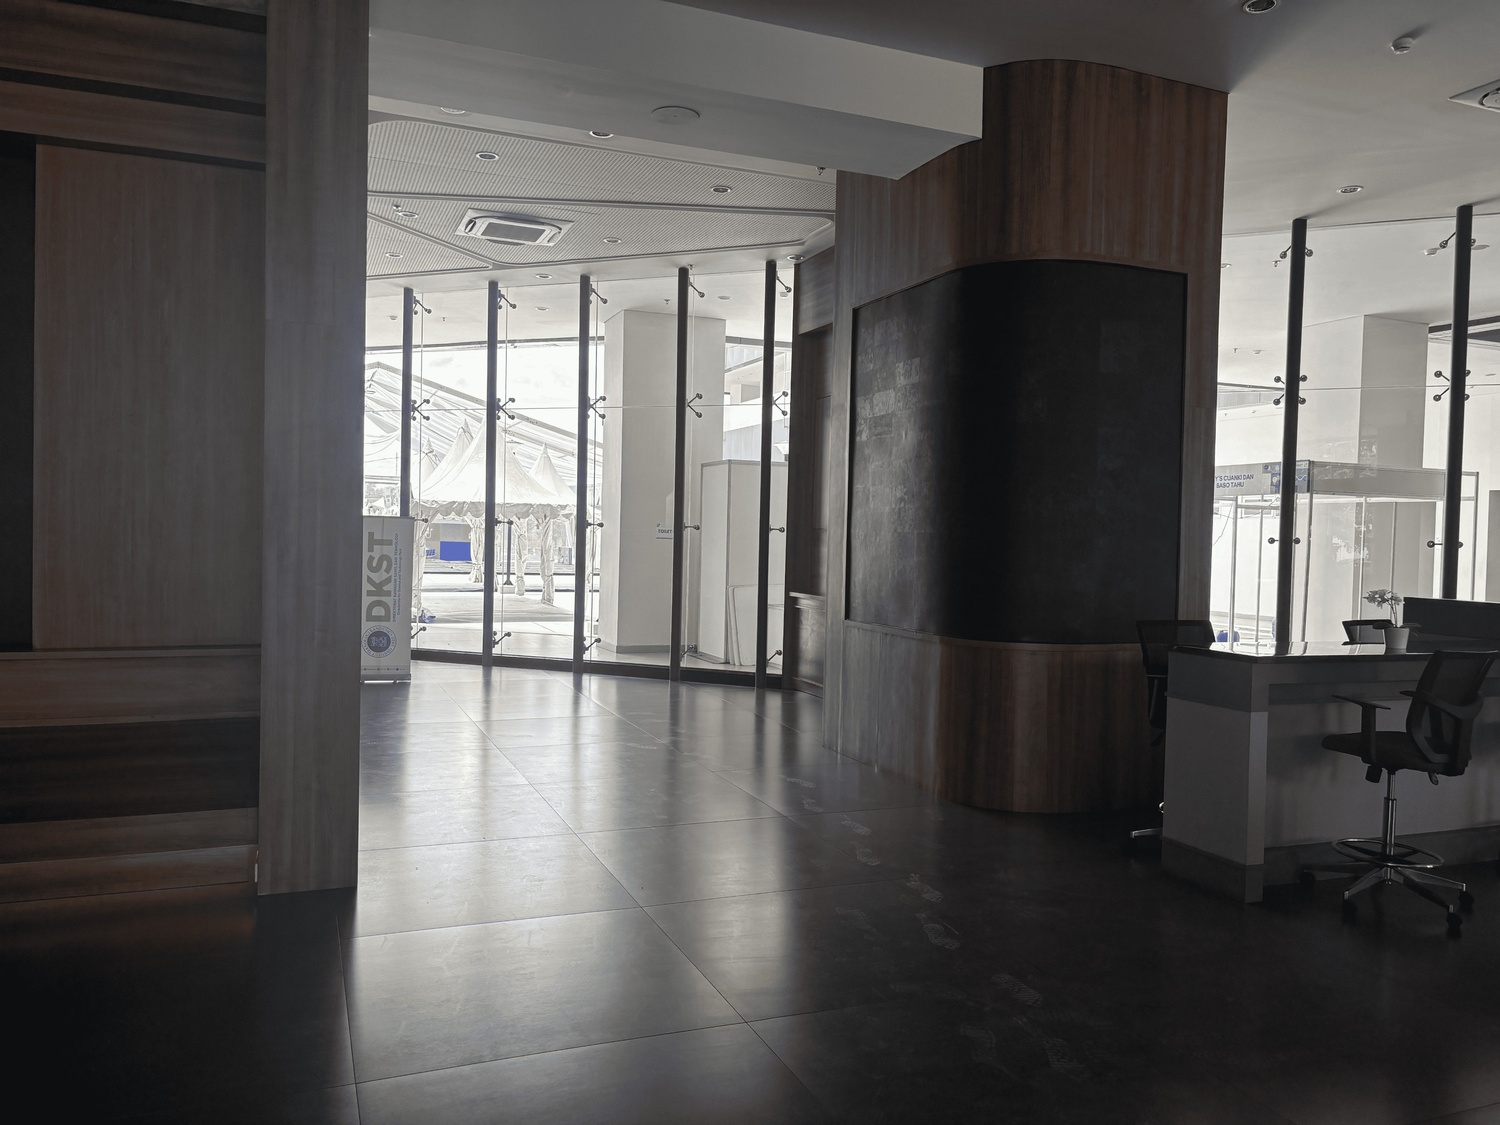
\includegraphics[width=0.6\textwidth]{images/wawancara1_1.png}
    \caption{Sesi Diskusi 1}
\end{figure}

\begin{figure}[htbp]
    \centering
    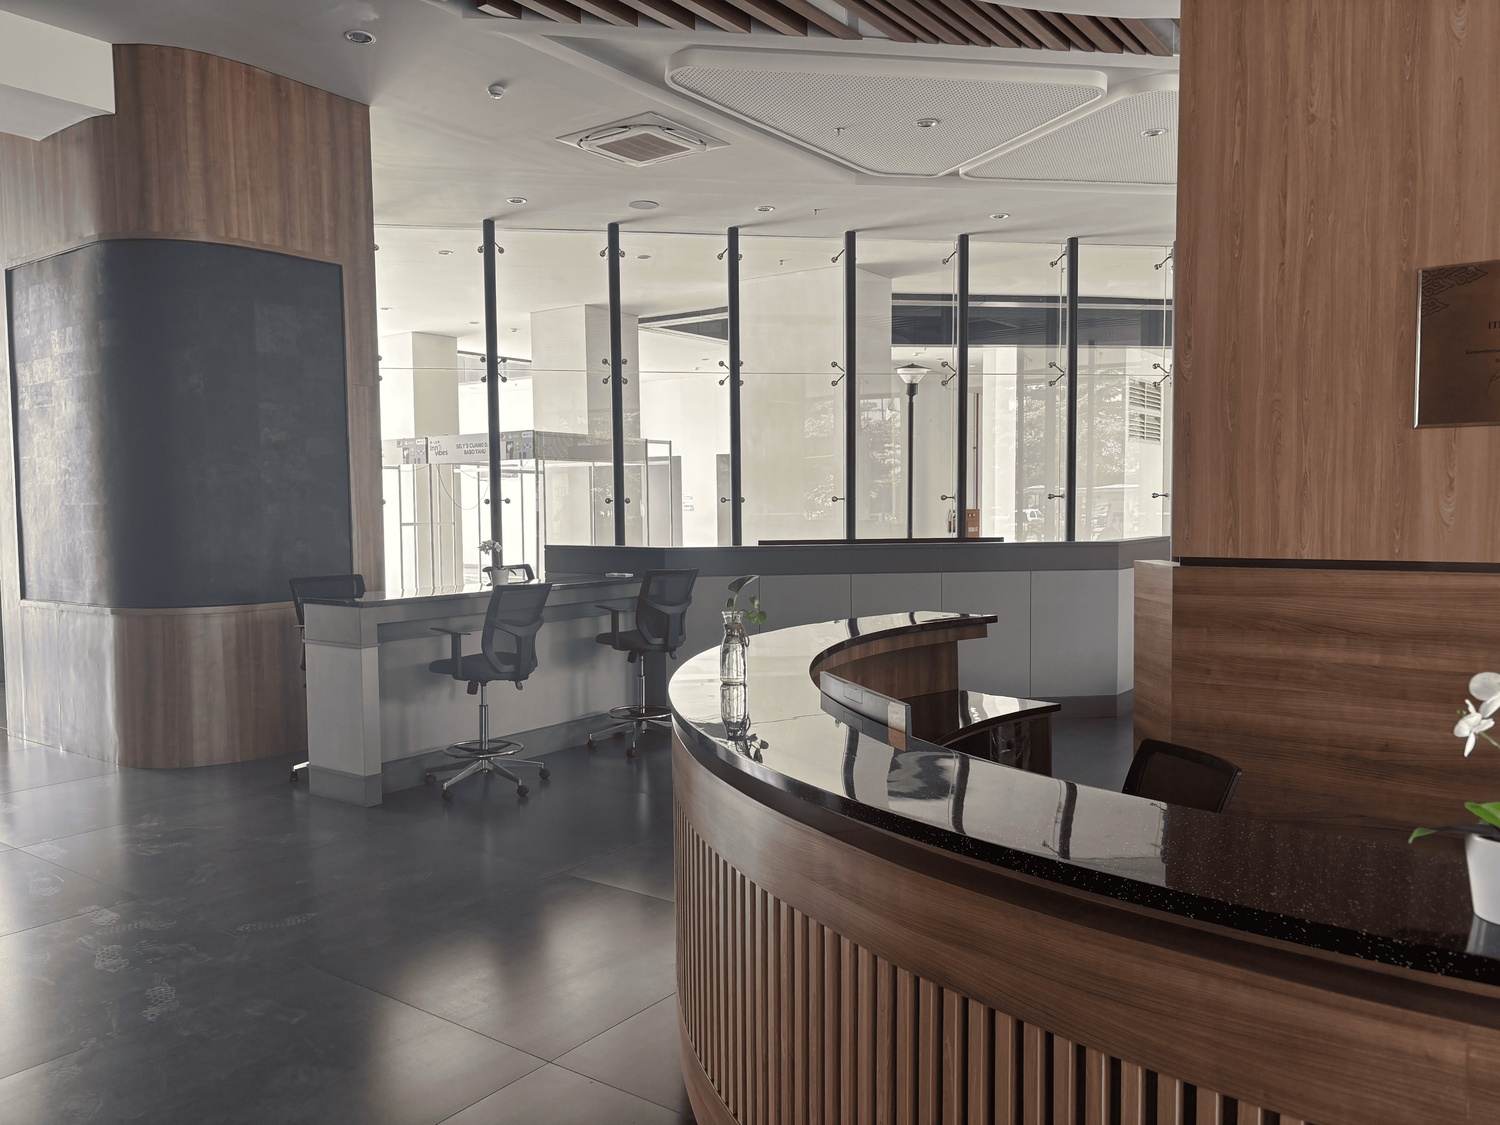
\includegraphics[width=0.6\textwidth]{images/wawancara1_2.png}
    \caption{Sesi Diskusi 2}
\end{figure}

\begin{figure}[htbp]
    \centering
    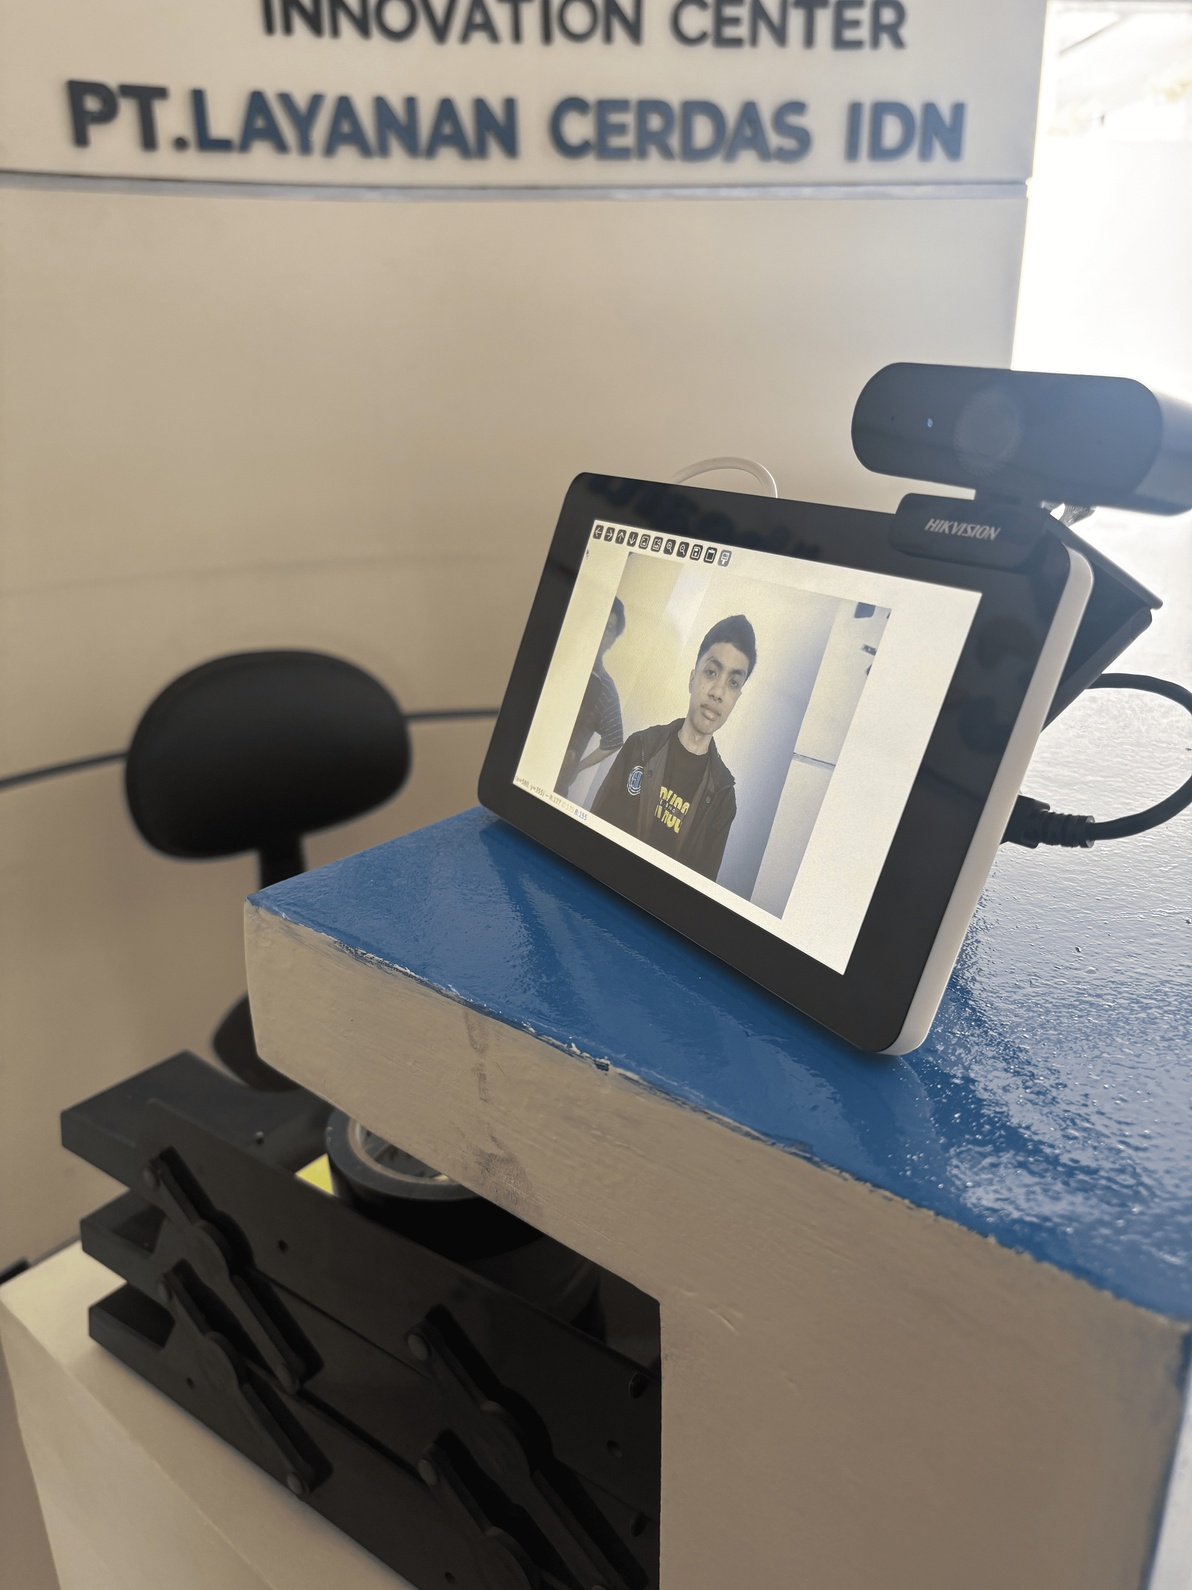
\includegraphics[width=0.6\textwidth]{images/wawancara1_3.png}
    \caption{Sesi Diskusi 3}
\end{figure}

\section{Transkrip Wawancara 1}
Wawancara dilakukan dengan pihak pengelola operasional Gedung ITB Innovation Park untuk menggali kebutuhan sistem dan memahami batasan operasional yang ada. Berikut adalah transkrip lengkap dari diskusi tersebut:

\begin{longtable}{|c|p{0.35\textwidth}|p{0.55\textwidth}|}
\hline
\textbf{No} & \textbf{Pewawancara (Mahasiswa)} & \textbf{Narasumber (Pengelola Gedung)} \\ \hline
\endfirsthead
\hline
\textbf{No} & \textbf{Pewawancara (Mahasiswa)} & \textbf{Narasumber (Pengelola Gedung)} \\ \hline
\endhead
\hline
\endfoot
\hline
\endlastfoot
1 & Kalau pengunjung atau karyawan masuk ke gedung, alur saat ini seperti apa, Pak? & Ya paling di lobi, Mas. Kalau di B1 naik ke B1, ya ke lantai-lantai yang mereka tuju. Rencananya akan dipasang kontrol akses di lobi, di B1, sama di akses lift. Dan di tiap-tiap pintu ruangan itu mau dipasang juga. \\ \hline
2 & Pengecekan security saat ini hanya mengecek apa saja? & Iya, cuman ngecek mau ke lantai berapa, tujuannya siapa, baru manual. Mungkin nanti kita pasangnya pakai face recognize. Jadi yang pengenalan wajah, sidik jari, sama RFID. \\ \hline
3 & Apakah IIP sebenarnya mau dijadikan gedung cerdas (Smart Building)? & Iya, masuknya ke konsep smart building sama green building. Kalau green building-nya kita udah 30\% on grid pakai solar panel listriknya. Terus kalau di segi air (water), air pengolahan masuk lagi ke pemakaian. \\ \hline
4 & Berarti sudah ada rencana pemasangan palang pintu (barrier) di lobi? & Iya, swing barrier. Rencananya kita lagi pemilihan vendor. Nah, si Mas aja yang pasang coba, itu kan tugas akhir. \\ \hline
5 & Untuk akses keluar masuknya (in/out) pakai pengenalan wajah? & Kalau pengenalan wajah lebih ke karyawan, terus tenant-tenant yang ada di atas. Kalau RFID lebih ke tamu-tamu. \\ \hline
6 & Menurut Bapak pribadi, ekspektasi performa dari swing barrier ini seperti apa? & Kalau performa kan itu lebih ke elektrik ya. Pembacaannya harus akurat maksimal di angka 90\%, terus fit in/out-nya yang memang nanti diatur. \\ \hline
7 & Apakah barrier dipasang untuk jalur masuk dan keluar? & Iya, di lobi sebelum masuk lift rencana kita pasang swing barrier di situ. Jaraknya 3,4 meter (as ke as), jadi tiga barrier yang akan dipasang. Tiap barrier punya face recognition tiga biji, berarti enam. Masuknya tiga, keluarnya tiga. \\ \hline
8 & Kalau di area basemen (B1 atau B2) rencananya bagaimana? & B1 pakai door access, pakai RFID atau face recognition juga bisa kan. Cuman kan bisa satu modul tuh RFID sama pengenalan wajah. \\ \hline
9 & Selain akses, apakah ada fitur tambahan yang diinginkan, misalnya untuk absensi? & Absen sekarang ada di bawah (lobi), di printer doang. Masing-masing punya absen sendiri di ruangan. Lantai 7 udah punya perusahaan sendiri, Prof. Trio. \\ \hline
10 & Bagaimana SOP pengecekan tamu masuk sebelum adanya sistem otomatis ini? & Orang datang misalkan di B1. Security catat nama dan kebutuhannya ke lantai berapa. Nanti dihubungi ke lantai tujuan via intercom, bisa diterima atau tidak. Kalau ke lobi langsung ke resepsionis, ditanya peruntukannya ke mana. Itu masih manual (old school). \\ \hline
11 & Jika dipasang sistem otomatis, apakah SOP akan berubah? & Nanti tamu KTP-nya ditukar kartu akses, kan enggak mungkin kita langsung akses mukanya karena hanya tamu. Kalau karyawan lebih enak pakai Face. Saya akan atur SOP-nya: security enggak pegang kartu RFID, tapi nge-tap pakai sidik jari mereka. \\ \hline
12 & Apakah saat ini sudah ada pusat data (data center) untuk sistem manajemen bangunan? & Sudah ada, Mas. Di sini masing-masing lantai ada server, dimasukin ke server data center. Sekarang sudah data pusat semua. \\ \hline
13 & Untuk fitur kehadiran, apakah lebih baik disatukan di lobi atau diurus masing-masing perusahaan tenant? & Karena ini gedung komersial, semua tenant punya ranahnya masing-masing. Biar mereka aja yang punya absen sendiri. Kapasitas face recognize kan ada maksimalnya, 1.500 sampai 3.000. Nanti kebanyakan juga pusing. \\ \hline
14 & Kira-kira berapa kapasitas maksimal karyawan/pekerja jika gedung ini penuh? & 1.200 orang maksimal. \\ \hline
15 & Apakah Bapak ada kebutuhan khusus atau ekspektasi fitur dari sistem yang akan kami buat? & Kebutuhan kita swing barrier. Nah, kalau ada ide dari kalian, ya ajuin aja. Kalian yang harus bisa improve apa yang bisa kita deploy di sini. Kalian yang mempunyai ide, apa yang akan kalian berikan masukan ke gedung ini. \\ \hline
16 & Kalau misalnya ditambahkan integrasi ke sistem alarm bencana, apakah boleh? & Kalau alarm kita sudah ada. Tapi swing barrier rencana sekarang belum terintegrasi ke kebencanaan. Kalau ada bencana misalkan barrier-nya dia buka, jadi enggak boleh ada kunci secara sistem. Bisa kan tambahin begitu. Tuh udah nemuin ide satu. \\ \hline
\end{longtable}
